\documentclass{article}
\usepackage{graphicx} % Required for inserting images
\usepackage{courier} %% Sets font for listing as Courier.
\usepackage{listings, xcolor}
\usepackage{exercise}

\usepackage{mathtools}
\usepackage{amssymb}
\usepackage{amsfonts}
\usepackage{graphicx}
\usepackage{float}
\usepackage{listings}
\usepackage{hyperref}
\usepackage{attachfile2}
\usepackage{vhistory}
\usepackage{epsfig}
\usepackage{subfig}
\usepackage{tikz}
\usetikzlibrary{external}
\tikzexternalize[prefix=tikz/]

\renewcommand\ExerciseName{Question~}
\renewcommand\AnswerName{Answer to question}
\renewcommand\ExerciseHeader{%
  \noindent\parbox[t]{.18\textwidth}{%
    \bfseries\large\ExerciseName\ExerciseHeaderNB\hfill}%
  \parbox[t]{.72\textwidth}{%
    \centering\bfseries\large%
    \ExerciseHeaderTitle\ExerciseHeaderOrigin}%
  \par\medskip
}

\newcommand{\addimg}[4]{
    \begin{figure}[H]
        \centering
        \includegraphics[#2]{#1}
    \caption{#3}
    \label{#4}
    \end{figure}
}

\lstset{
tabsize = 4, %% set tab space width
showstringspaces = false, %% prevent space marking in strings, string is defined as the text that is generally printed directly to the console
numbers = left, %% display line numbers on the left
commentstyle = \color{green}, %% set comment color
keywordstyle = \color{blue}, %% set keyword color
stringstyle = \color{red}, %% set string color
rulecolor = \color{black}, %% set frame color to avoid being affected by text color
basicstyle = \small \ttfamily , %% set listing font and size
breaklines = true, %% enable line breaking
numberstyle = \tiny,
}

\newcommand{\commitHash}{\href{https://github.com/fnieri/LanguagesAndTranslatorsTP/tree/c3a4f2f}{c3a4f2f}}
\newcommand{\commitDate}{2025-06-01}


\title{Language And Translators - TP Correction}
\author{Francesco Nieri}
\date{June 2024 (last update: \commitHash \  on \commitDate)}

\begin{document}
\maketitle
\tableofcontents
\newpage
\section{TP1}
    \input{TPs/tp1}
\newpage
\section{TP2}
    \input{TPs/tp2}
\newpage
\section{TP3}
    \input{TPs/tp3}
\newpage
\section{TP4}
    \input{TPs/tp4}
\newpage
\section{TP5}
    \input{TPs/tp5}
\newpage
\section{TP6}
    \subsection{Question 1}
    \textbf{Give the intermediate representation in TAC for the following expression:}

    \input{TP6/q1}

    \input{TP6/1}

\subsection{Question 2}
    \textbf{For each of the following C functions, give the control flow graph (CFG), the minimized SSA form, and the non-SSA form without parameterized labels (the form that can be used to generate assembly code)}

    \input{TP6/q2}
    \begin{figure}[H]%
                \centering
                \subfloat[\centering]{{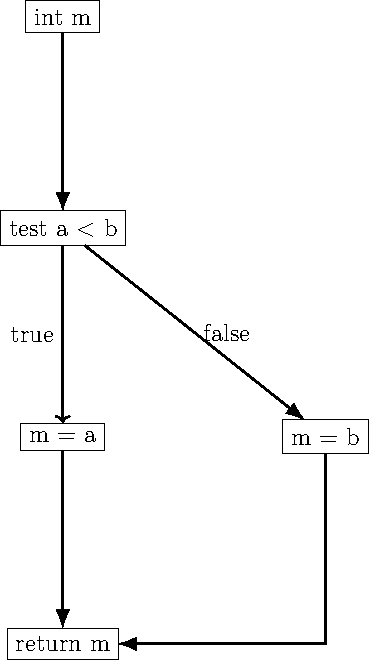
\includegraphics[width=5cm]{img/TP6/cfg_min.pdf} }}%
                \qquad
                \subfloat[\centering ]{{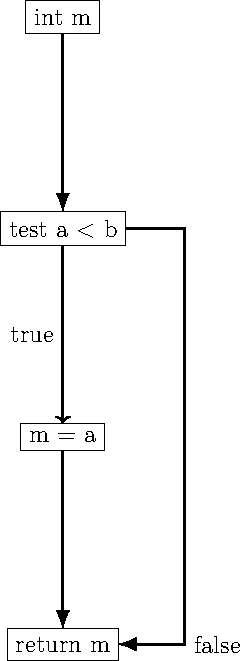
\includegraphics[width=5cm]{img/TP6/cfg_min_alternative.pdf} }}%
                \caption{CFG for min and minAlternative $(a|b|bc)^{*}a$}%
                \label{fig:example}%
            \end{figure}
    \addimg{img/TP6/cfg_squareSum.pdf}{scale=0.5}{CFG for squareSum}{}
    
    Minimized SSA for min:
    \begin{lstlisting}[language = Java , frame = trBL , firstnumber = last , escapeinside={(*@}{@*)}]
min(a0,b0):
    if a0 < b0 then goto body else goto elsebody
body:
    m0 = a0
    goto done(m0)
elsebody:
    m1 = b0
    goto done(m1)
done(m2):
    return m2
\end{lstlisting}
    Minimized SSA for minAlternative:
    \begin{lstlisting}[language = Java , frame = trBL , firstnumber = last , escapeinside={(*@}{@*)}]
minAlternative(a0,b0):
    m0 = b0
    if a0 < b0 then goto body else goto done(m0)
body:
    m1 = a0
    goto done(m1)
done(m3):
    return m3
\end{lstlisting}
    Non minimized SSA for squareSum:
    \input{TP6/square_sum_nm_ssa}
    Minimized SSA
    \input{TP6/square_sum_min_ssa}
    Non minimized non-SSA
    \input{TP6/square_sum_non_ssa}
    Minimized non-SSA
    \input{TP6/square_sum_min_non_ssa}

\subsection{Question 3}
    \textbf{Design a simple algorithm that verifies that a function has no missing return statement. The algorithm should also work for complex functions that contain many if-statements, loops, etc.}

    \input{TP5/3}


\newpage
\section{TP7}
    \input{TPs/tp7}
\end{document}
